% Compile with XeLaTeX or LuaLaTeX, twice for cross-references.
% Change 169 to 43 here for a traditional 4:3 canvas.
\providecommand{\BeamerAspectRatio}{169}
\documentclass[aspectratio=\BeamerAspectRatio]{beamer}
\usetheme{LeipzigClean}
% Replace these fields for each presentation.
\title[Umgang mit KI]{Wie man KI (richtig) einsetzt}
\subtitle{Chancen, Risiken und die Rolle des Menschen}
% Name and affiliation can be entered here before presenting.
\author{Jonas}
\institute{}
\date{Feierabendseminar 08.10.2026}
\titlegraphic{}
% Optional link beneath the title metadata:
% \titlegraphic{\small\color{Muted}\href{https://example.org}{Project website}}

\usepackage[backend=bibtex,style=authoryear,maxcitenames=2,maxbibnames=9,natbib=true,doi=true,url=false,isbn=false]{biblatex}
\addbibresource{references.bib}

\begin{document}
\maketitlepage
% Optional overview: uncomment when the talk has multiple sections.
% \maketableofcontents
% Optional section dividers: comment out the next line to hide them.
% \makesectionpopup

\section{Umgang mit KI}\label{sec:ki}

\subsection{Motivation}
\begin{frame}{KI wird immer relevanter}

\end{frame}

\subsection{Arten von KI-Nutzung}
\begin{frame}{Arten von KI-Nutzung}
  \keyidea{Es gibt unendliche viele Arten, KI zu nutzen.}
  \begin{itemize}
    \item Sentence-Transformer - Kosinus-Rechnung für Ähnlichkeitsanalyse
    \item Chatbot: Wiki, Tutor, Literaturrecherche, persönliche Assistenz
    \item Bildgenerierung: Erstellung von Grafiken, Diagrammen oder Illustrationen
    \item Datenanalyse: Unterstützung bei der Auswertung und Visualisierung von Daten
    \item Codegenerierung und Debugging
    \item Agentische KI: komplexe Aufgaben automatisiert ausführen lassen
  \end{itemize}
\end{frame}

\subsection{Sinnvoller Einsatz von KI-Tools}
\begin{frame}[fragile]{Sinnvoller Einsatz von KI-Tools (Stand vor ein paar Monaten)}
    \footnotesize
    KI-Sprachmodelle sind mächtige Werkzeuge, aber nicht für jeden Schritt im Forschungsprozess gleichermaßen geeignet.

    \vspace{0.5em}
    \begin{myalert}{Wo Vorsicht geboten ist (Eine immer obsoletere Liste von diesem Sommer)}
        \begin{itemize}
            \item \textbf{Zusammenfassung von Papern:} Meist unnötig, da der Abstract diese Aufgabe ohnehin schon optimal erfüllt.
            \item \textbf{Erklärung  Begriffe:} Gut für den Einstieg, vermittelt jedoch oft kein tieferes wissenschaftliches Verständnis.
            \item \textbf{Literaturrecherche:} Nützlich für einen ersten Überblick, der tatsächliche Einblick in die relevanten Arbeiten muss aber zwingend selbst passieren. Oft sind Review/Übersichts-Artikel eine bessere Anlaufstelle. 
        \end{itemize}
    \end{myalert}

    \begin{mynote}{Wo KI ihre Stärken voll ausspielt (Inzwischen eine viel kleinere Liste als sie sein sollte)}
        \begin{itemize}
            \item \textbf{Textproduktion:} Eigene, rohe Stichpunkte in flüssige Textpassagen ausformulieren lassen.
            \item \textbf{Klar definierte Aufgaben:} Allerlei kleine Handgriffe, zum Beispiel komplexe Formeln ausschreiben, \LaTeX-Befehle generieren oder Python-Code schreiben.
            \item Oberflächliche Überarbeitung und Debugging von Text und Code
            \item Übersetzungen, Synonyme und alternative Formulierungen 
        \end{itemize}
    \end{mynote}
\end{frame}

\begin{frame}{Agentische KI-Tools}
  \begin{columns}
    \column{0.5\textwidth}
    \begin{mynote}{Nutzungsmöglichkeiten}
    \begin{itemize}
        \item Erstellung interaktiver Lernumgebungen
        \item technische Umsetzung von Spielideen
        \item Einrichtung von automatisierten KI workflows wie Paper parsing
        \item Templates Erstellen
        \item Komplexe Graphiken, z.B. mit Tikzpictures
    \end{itemize}    
  \end{mynote}
  \column{0.5\textwidth}
  \centering
  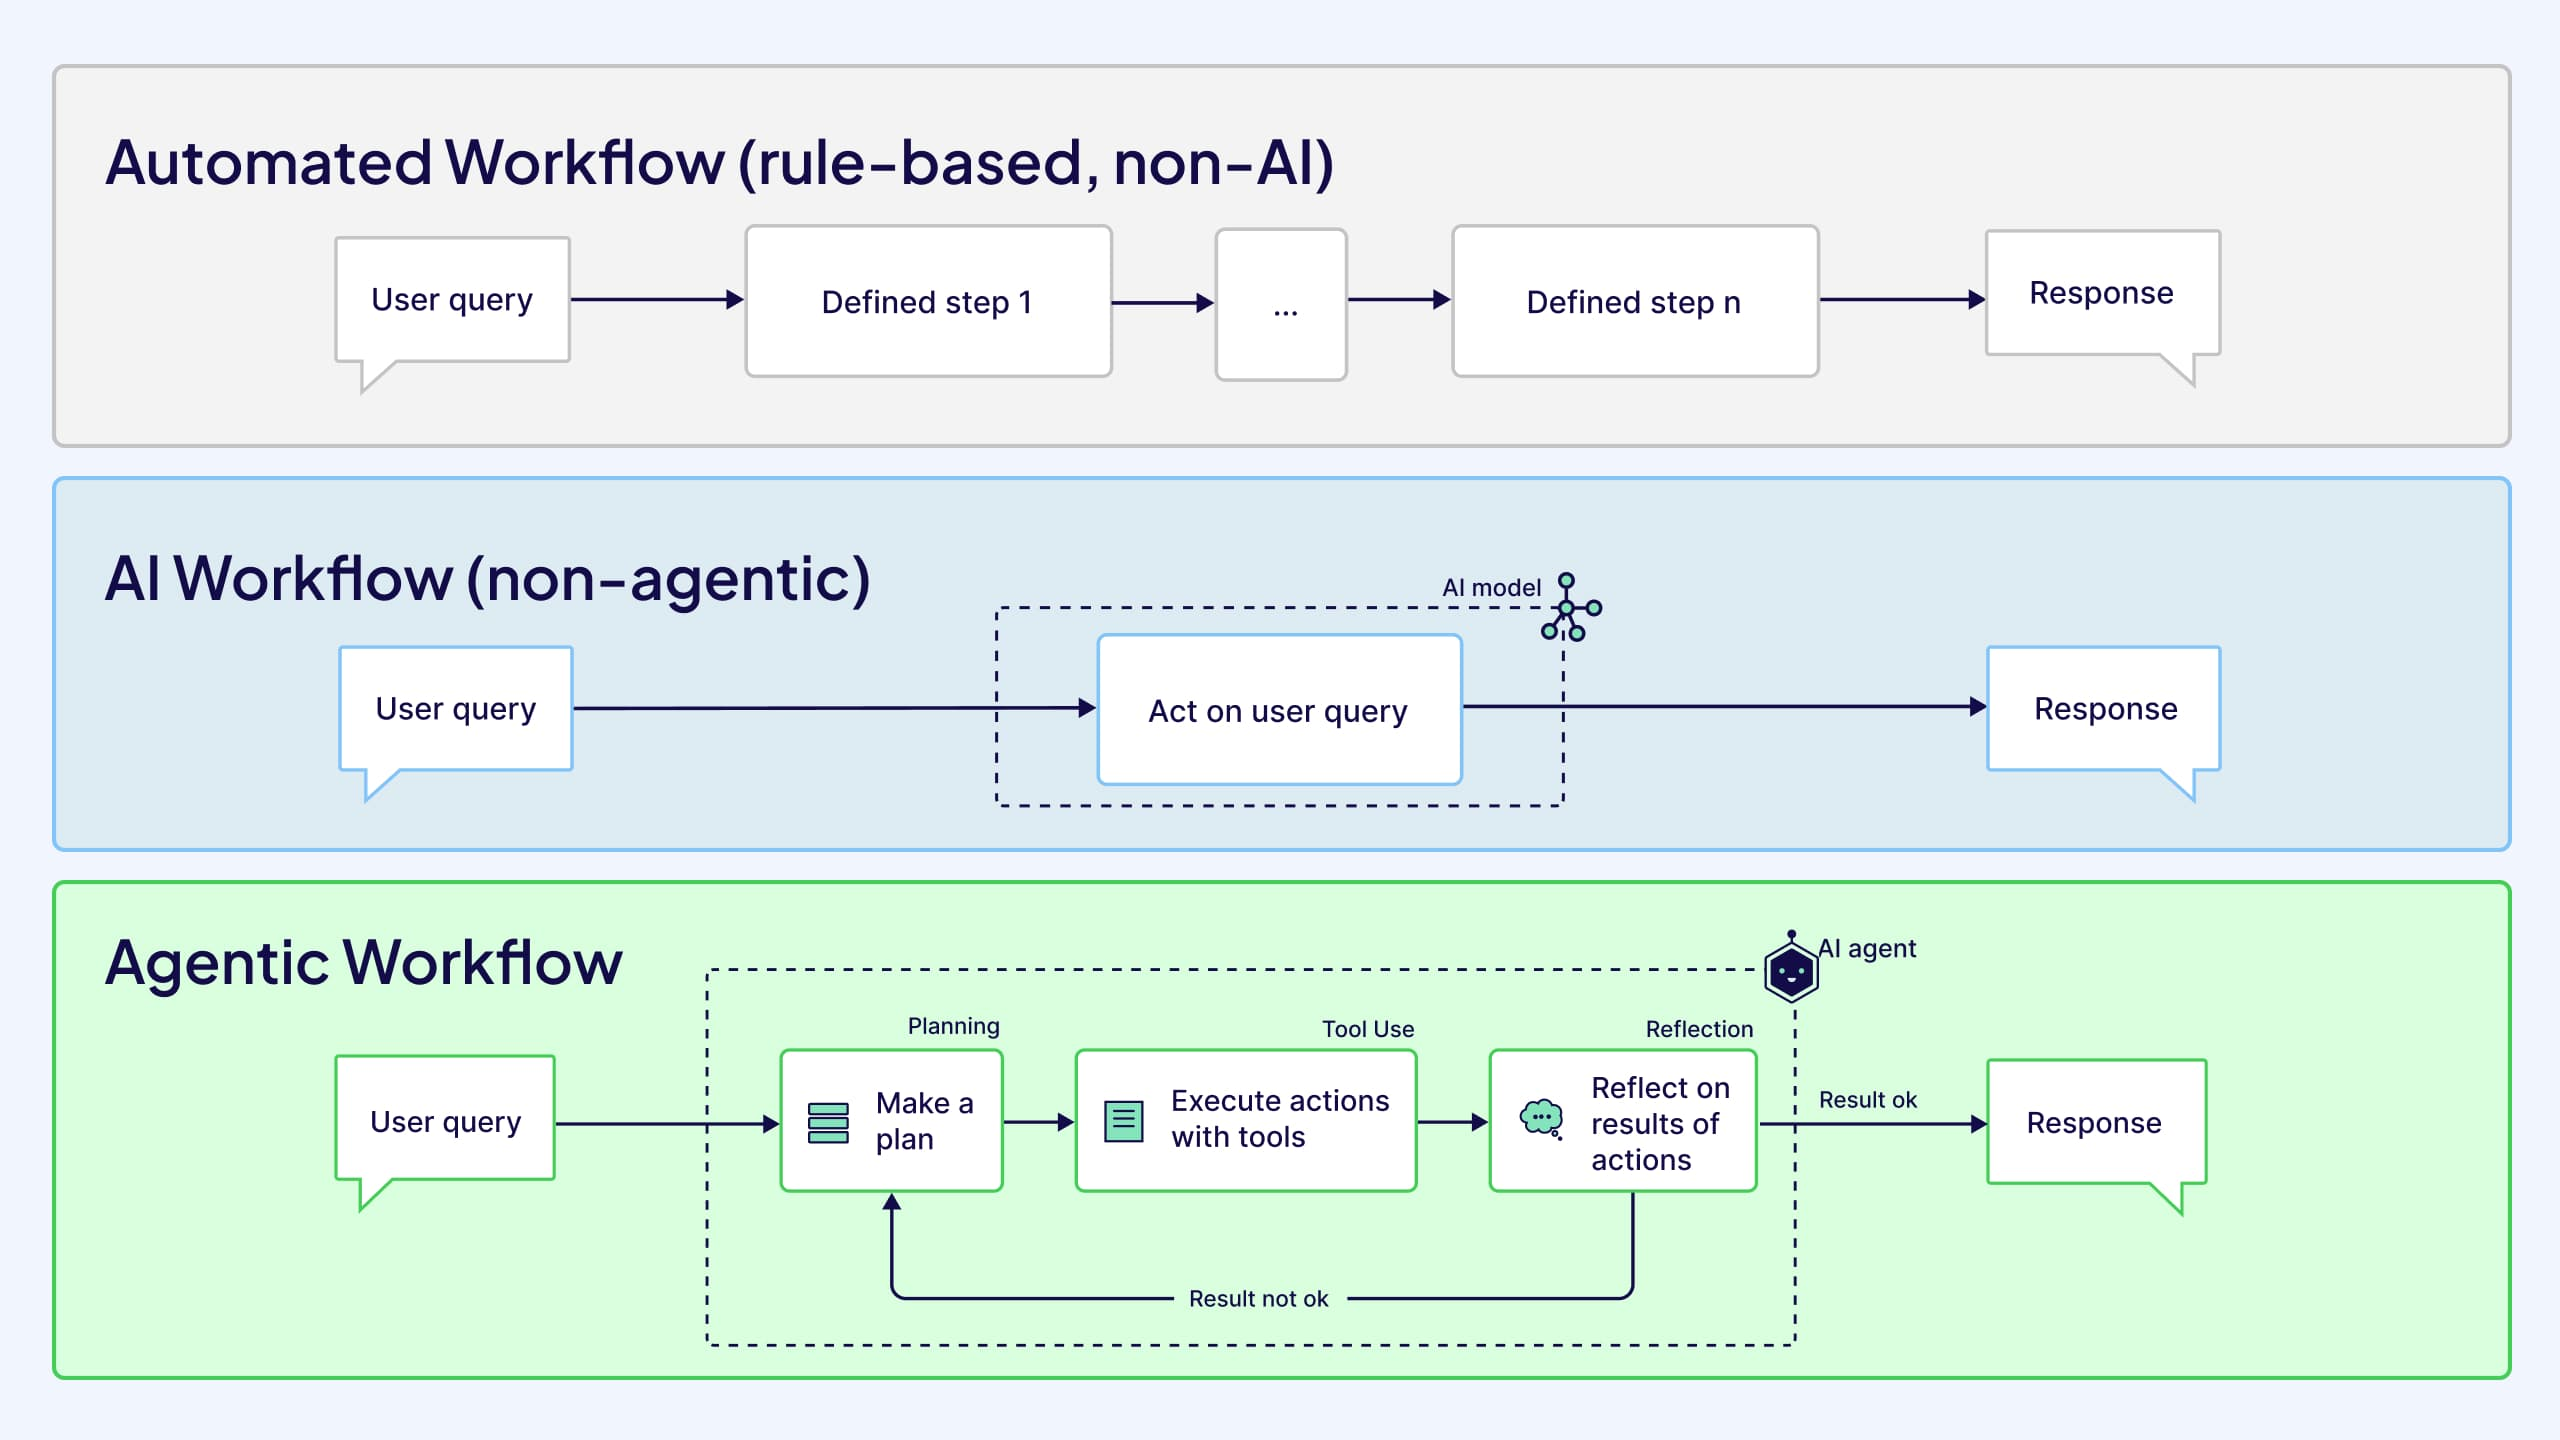
\includegraphics{images/agentic_workflow.png}
  \source{\url{https://weaviate.io/blog/what-are-agentic-workflows}}
  \end{columns}
\end{frame}

\begin{frame}{Die eigentlichen Probleme}
    \begin{myalert}{Output-Orientierung}
        \begin{itemize}
          \item Es ist sehr menschlich Dinge zu mögen, die KI generiert: Es ist designt dazu gut zu klingen, und inzwischen auch qualitativ überzeugend.
          \item Besseren Output erzielt man, wenn man KI verwendet $\to$ es entsteht eine Erwartungshaltung bzgl. Produktivität
          \item Was KI aber nicht kann: Arbeiten ohne Output-Orientierung. 
        \end{itemize}
    \end{myalert}
    \begin{myalert}
      \begin{itemize}[Kulturelles \& Soziales]
          \item Goodhart's Law: Wenn ein Maß zum Ziel wird, hört es auf ein gutes Maß zu sein. Für KI ist aber das Maß das einzige Ziel.
          \item Verwaschung menschlichen Wissens $\to$ Spezialwissen wird immer wichtiger.
          \item Menschliche Fähigkeiten nehmen ab durch die Nutzung von KI: wo wollen wir unsere Fähigkeiten bewahren?
      \end{itemize}
    \end{myalert}
    \keyidea{Die menschliche Motivation ist entscheidend.}
\end{frame}

\subsection{Die Rolle des Menschen}
\begin{frame}{Umgang mit KI: Die Rolle des Menschen}
\begin{columns}[T,onlytextwidth]
\column{0.46\textwidth}
\begin{figure}
    \centering
    \includegraphics[width=0.9\linewidth]{astra.png}
    \caption{Recent advances by Astra \cite{openai_ten_advances}}
    \label{fig:placeholder}
\end{figure}\column{0.54\textwidth}
            \begin{figure}
                \centering
                \includegraphics[width=\linewidth]{math_knowledge.png}
            \end{figure}
            \begin{figure}
                \centering
                \includegraphics[width=\linewidth]{problem_solving.png}
                \caption{Mathematical Problem Solving Processes \cite{tao_ai_2026}}
                \label{fig:problem_solving}
            \end{figure}
\end{columns}
\end{frame}

\begin{frame}{Die goldene Regel und das FERC framework}
    \footnotesize  
    \metroset{block=fill}
    \begin{myalert}{Die goldene Regel}
        Die allerbesten Ergebnisse bekommt man, wenn man präzise beschreibt und \textbf{selbst genau weiß, was man will!}
    \end{myalert}
    \vspace{-0.7em}
    \metroset{block=transparent}
    \begin{columns}[T]
        \column{0.5\textwidth}
        \begin{mynote}{Das FERC Framework \cite{ferc}}
            \begin{description}[Explore]
                \item[Frame] Menschlichen Kontext, Ziele und Grenzen formulieren. KI durch Klarheit auf Erfolg ausrichten.
                \item[Explore] KI-Optionen durch gezieltes Prompting generieren. Verschiedene Ansätze erkunden und vergleichen.
                \item[Refine] Iteration durch menschliches Feedback und Evaluation. Co-Kreation durch systematische Verbesserungszyklen.
                \item[Commit] Finale Entscheidung basierend auf menschlichem Urteil treffen. Der Mensch verantwortet das Ergebnis.
            \end{description}
        \end{mynote}
        
        \column{0.5\textwidth}
        \begin{mynote}{Anwendungsprinzipien}
            \begin{enumerate}
                \item Niemals die KI den ersten Entwurf liefern lassen -- immer Kontext und Struktur vorgeben.
                \item KI nicht als Expertenwissen über die eigene (oder die der Organisation) Expertise hinaus nutzen.
                \item FERC nutzen, wenn menschliche Autorenschaft wichtig ist.
                \item Die Interaktion in ausreichend kleine Schritte unterteilen, damit das Abfragen von Optionen sinnvoll bleibt.
                \item Kleine Schritte bedeuten weniger Energieverbrauch und Kosten.
            \end{enumerate}
        \end{mynote}
    \end{columns}
\end{frame}

\begin{frame}{Anwendungsbeispiel: Vortrag vorbereiten zum Thema Künstliche Intelligenz}
\textbf{bad prompt:} Schreibe einen Vortrag zum Thema Künstliche Intelligenz

\textbf{bad prompt:} Bereite einen Vortrag zum Thema Künstliche Intelligenz vor, indem du zunächst die wichtigsten Punkte und eine Gliederung erstellst.

\textbf{okay prompt:} Schreibe einen Prompt, der zu einem informativen und gut strukturierten Vortrag führt. (Danach den Prompt reviewen und anpassen)

\textbf{okay prompt:} Mache einen Vorschlag für eine Vortragsstruktur und ein paar Schlüsselideen, die ich in meinem Vortrag zu den Umgang mit KI und den zugehörigen Risiken verwenden könnte.

\textbf{good prompt:} Ich möchte in meinem Vortrag folgende Schlüsselideen rüberbringen:
\begin{itemize}
\item KI wird immer besser in allem $\to$ es ist keine Debatte mehr, dass sie menschliche Fähigkeiten in vielen Bereichen obsolet macht.
\item Output-Orientierung ist das zentrale Funktionsprinzip und gleichzeitig eines der größten Probleme.
\item Informationsüberfluss und Produktivitätssteigerung führen zu Verwaschung menschlichen Wissens und Leistungsdruck.
\item Menschliche Motivation und Intention ist entscheidend für den verantwortungsvollen Einsatz von KI.
\item Das FERC-framework ist ein erster Ansatz, um \glqq on-top \grqq zu bleiben.
\end{itemize}
Verwende bitte folgendes Template: github link. Mache Vorschläge, wo ich Schlagzeilen und Bilder einsetzen könnte und wo ich die Punkte mit der verfügbaren Fach-Literatur unterstützen kann. 
\textbf{good prompt:} Ich habe folgenden Vortrag geschrieben [Link zu Projekt-Ordner]. Die Motivationsfolie soll verschiedene Schlagzeilenmäßig nacheinander einblenden (aktuell 10_advances, astra, navier_stokes, hugging_face, 727_papers in der Reihenfolge) und dabei sollen die sich überlappen. Hast du noch weitere vorschläge? Folie xx braucht noch ein Schaubild, das die Argumente in einem Flussdiagramm verknüpft. Erstelle das bitte mit tikzpictures. Ich suche noch Literatur zu den Gefahren von KI, kannst du gute Fachliteratur empfehlen? 
Ich suche noch Literatur zu den Gefahren von KI und weitere Ideen für die Nutzung agentischer KI-tools, bitte empfehle dazu Fachliteratur und was ich noch ergänzen könnte auf den entsprechenden Folien. Ich brauche noch eine Folie, die visuell (tikzpictures) das angefügt Paper von Terence Tao zusammenfasst und die Rolle des Menschen im wissenschaftlichen Prozess hervorhebt. Folie xy hätte ich gern in einem Stil, wo links rot hervorgehobener Text ist und rechts jeweils die Erklärung. Mache gern weitere Vorschläge, was man am Vortrag noch anpassen könnte. Im Allgemeinen soll natürlich alles auf die Folien passen und kompilieren. Vermeide es, zu verbös zu sein.
\keyalert{Sämtliche Outputs müssen reviewt und verstanden werden: sei nicht wie OpenAI und veröffentliche nicht Dinge, die du nicht verstehst.}

Hilfreicher Tipp: Am Ende nochmal eine Aufgabe finden, die einen dazu zwingt, den ganzen Text durchzugehen. Zum Beispiel, das Nacheinander-Einblenden der Punkte für einen Vortrag selbst machen. Abschnitte neu denken, bei denen man ein mulmiges Gefühl hat. Visualisierungen selbst erstellen. Im Allgemeinen lohnt es sich, auszuprobieren, was KI so kann!
\end{frame}

\subsection{Die Leiden Declaration}
\begin{frame}[fragile]{Umgang mit KI: Die Leiden-Erklärung}
    \footnotesize
    Die \textbf{Leiden Declaration (2026)} umfasst 11 Kernaussagen zum verantwortungsvollen KI-Einsatz. Teil 1 fokussiert sich auf Publikationspraxis:

    \vspace{0.5em}
    \begin{exampleblock}{Transparenz, Autorenschaft \& Review}
        % Schöne und kompakte Formatierung mit enumitem
        \begin{description}
            \item[01] \textbf{Offenlegung:} Einsatz von KI-Tools (LLMs, Beweisassistenten) transparent in Publikationen und bei Gutachten deklarieren.
            \item[02] \textbf{Review-Prozess:} Peer-Reviewern die Arbeit durch Offenlegung der KI-Nutzung, exakte Referenzen und formale Beweise erleichtern.
            \item[03] \textbf{Open Science:} Prinzipien der offenen Wissenschaft befolgen, um Forschungsergebnisse für alle transparent und zugänglich zu machen.
            \item[04] \textbf{Verantwortung:} Die \textit{ausschließliche} Verantwortung für die Richtigkeit der Argumente, Ergebnisse und Zitate verbleibt beim Menschen.
            \item[05] \textbf{Autorenschaft:} Credits gehören dem Menschen, nicht der Maschine; KI kann die kollektive menschliche Leistung nicht ersetzen.
            \item[06] \textbf{Quellenarbeit:} Aufgrund von KI-Schwächen proaktiv nach Originalquellen suchen und diese sorgfältig und korrekt zitieren.
        \end{description}
    \end{exampleblock}
\end{frame}

\begin{frame}[fragile]{Umgang mit KI: Die Leiden-Erklärung}
    \footnotesize
    Teil 2 der Erklärung adressiert unsere Rolle in der wissenschaftlichen Gemeinschaft und der Gesellschaft:

    \vspace{0.5em}
    \begin{exampleblock}{Gemeinschaft, Ethik \& Gesellschaft}
        \begin{description}
            \item[07] \textbf{Öffentlicher Diskurs:} Sich aktiv einbringen, um KI-Methoden einzuordnen und fundierten Wissenschaftsjournalismus zu unterstützen.
            \item[08] \textbf{Weiterbildung:} Sich kontinuierlich über die Fähigkeiten und Grenzen neuer computergestützter Werkzeuge informiert halten.
            \item[09] \textbf{Neue Mitwirkende:} Interdisziplinäre Beiträge begrüßen und eigene Standards zugänglich machen, um Neueinsteigern den Weg zu erleichtern.
            \item[10] \textbf{Werkzeugwahl:} Tools kritisch prüfen und bevorzugt nicht-proprietäre oder ressourcenschonende Alternativen nutzen.
            \item[11] \textbf{Ethik:} Gesellschaftliche Folgen der eigenen Arbeit evaluieren und bei schädlichen Anwendungen (Überwachung, Krieg) Konsequenzen ziehen.
        \end{description}
    \end{exampleblock}
\end{frame}

\begin{frame}[fragile]{Der problematische Ressourcenverbrauch durch KI}

\begin{figure}
    \centering
    \includegraphics[width=0.85\linewidth]{bilder/ai_energy_market_dynamics.png}
    \caption{AI energy-market dynamics \cite{Alpine2026}.}
\end{figure}

\end{frame}

\begin{frame}[fragile]{Der problematische Ressourcenverbrauch durch KI}

\begin{figure}
    \centering
    \includegraphics[width=0.7\linewidth]{bilder/ai_mediated_productivity.png}
    \caption*{Jährliche CO2-Emissionen durch KI heute und 2035 \cite{Alpine2026}.}
\end{figure}

\end{frame}

\begin{frame}[allowframebreaks]{References}
\renewcommand*{\bibfont}{\scriptsize}
\printbibliography
\end{frame}

% Optional appendix. Disable divider pages for backup material.
% \appendix
% \AtBeginSection[]{}
% \begin{frame}{Additional details}
%   Supporting material goes here.
% \end{frame}

\end{document}
